\documentclass[9pt]{beamer}
\mode<presentation>
% input and font settings
\usepackage[utf8]{inputenc}		% for UTF8 input
\usepackage[T1]{fontenc}			% for T1 font family
\usepackage[english]{babel}		% for multilanguage input
% other settings
\usepackage{mathtools}
\usepackage{varwidth}
\usepackage{xcolor}
\usepackage{xfrac}
\usepackage{mathabx}
\usepackage[export]{adjustbox}
\usepackage{pgffor}
\usepackage{etoolbox}
\usepackage{xstring}
\usepackage{siunitx}
\usepackage{epstopdf}			% convert images to png
\epstopdfDeclareGraphicsRule{.tif}{png}{.png}{convert #1 \OutputFile}		% to covert TIF to PNG automatically
\AppendGraphicsExtensions{.tif}
%%% beamer settings
\beamertemplatenavigationsymbolsempty
%\usetheme{Boadilla}
\usetheme{Frankfurt}
\makeatletter
\@removefromreset{subsection}{section}
\makeatother
\setcounter{subsection}{1}



%%% author information
\author{Daniel \v{S}m\'{i}t}
\title{Crawling in the books}

\setbeamertemplate{itemize items}[default]
\setbeamertemplate{enumerate items}[default]

%%% document starts here
\begin{document}

%%% title frame
\begin{frame}{}
	\centering\Large
	\vspace{1em}
	{Crawling in the books\\}
	\vspace{1em}
	{Daniel \v{S}m\'{i}t\\}
	\vspace{1em}
\end{frame}

%%% the first section of slides
\section{Preparation}

\begin{frame}{Initial insights}
	Filter the data, gain initial insights
	\begin{itemize}
		\item clean bad data, remove lone ratings: user with 1 book, book with 1 rating
		\item filter LOTR books (keep other Tolkien books for validation), compute rating count and mean rating
		\item plot ratings by age (bell), geolocation (USA), \structure{ratings count per user}
	\end{itemize}
	\begin{figure}
		\centering
		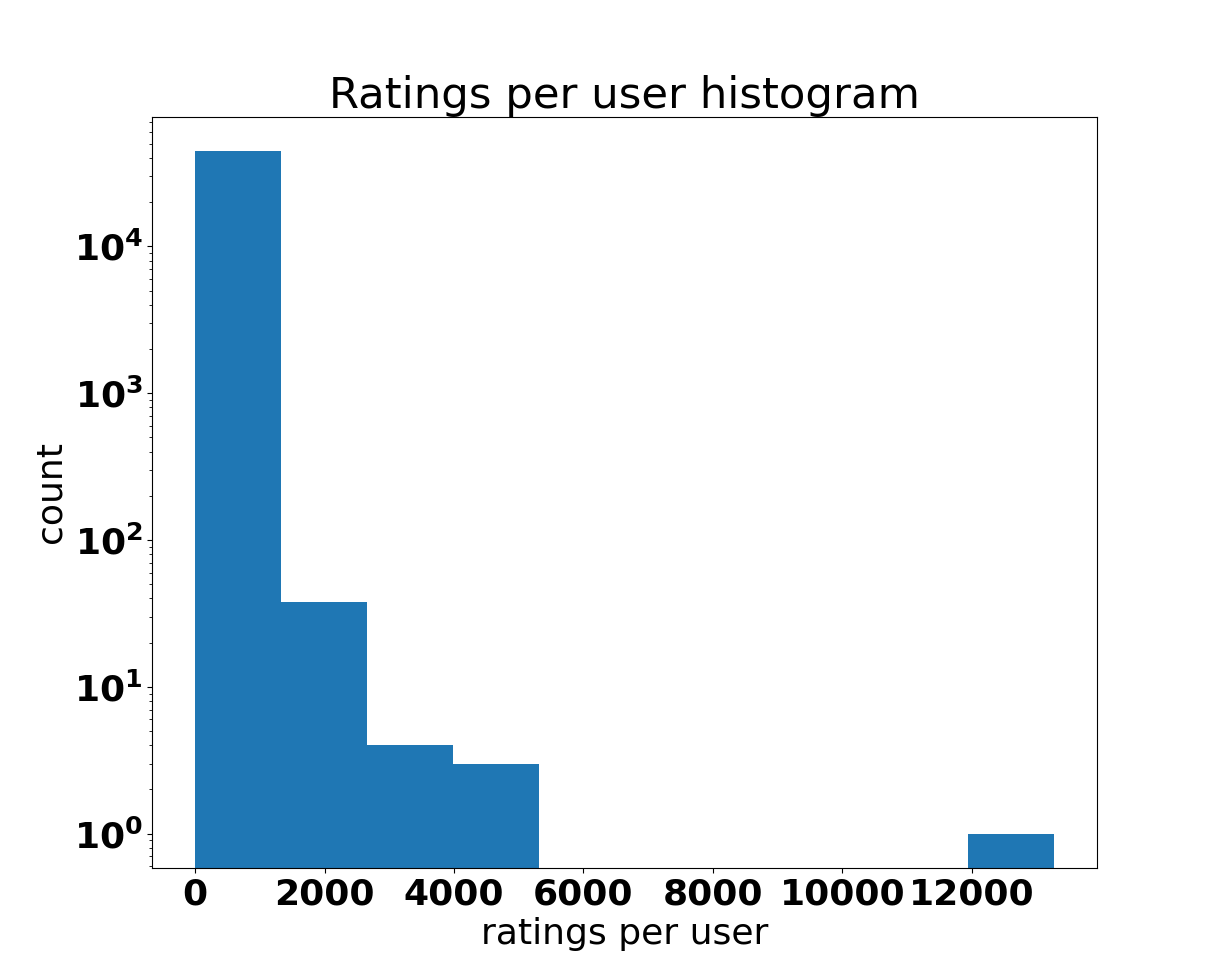
\includegraphics[width=0.7\textwidth]{../img/user-hist.png}
		\caption{User rating count histogram}
	\end{figure}
\end{frame}

%%% the second section
\section{Metrics}

\begin{frame}{Rating group processing}
	Process user-based groups
	\begin{itemize}
		\item select user-based rating groups $\{\gamma_i\}$ which contain at least one LOTR book
		\item \emph{count LOTR books} $\{\lambda_i\}$ and \emph{count all books} $\{\beta_i\}$ in each user group $i$ 
		%\item remove LOTR books from those groups 
	\end{itemize}
	Prepare metrics for each relevant book
	\begin{enumerate}
		\item book belongs to $J>5$ rating groups $\{\gamma_1,\ldots,\gamma_J\}$ 
		\item mean number of LOTR books co-ocurring in rating groups $\Lambda =\frac{1}{J}\sum_{j=1}^{J} \lambda_j $
		\item mean size of rating groups $B = \frac{1}{J}\sum_{j=1}^J \beta_j$
		\item book weight as $W = \frac{\Lambda}{B}$
	\end{enumerate}
	Weight add importance to groups where a book is accompanied by a large proportion of LOTR/Tolkien books.\\
	Note that we could have chosen another metric for weight, possibly involving mean rating, or rating std.
\end{frame}

\begin{frame}{Ranking}
	Ranking of Tolkien co-rated books:\\
	\begin{itemize}
		\item compute weighted count $\kappa=W\cdot J$ of each book belonging to $\{\gamma_1,\ldots,\gamma_J\}$
		\item rank book within Tolkien co-rated set $\{\gamma_i\}$ by $\kappa$
		\item rank all general books by their count $\kappa'$ in all ratings
		\item compute rank-gain for each book in Tolkien co-rated set $\kappa - \kappa'$ 
	\end{itemize}
	The rank gain represents how much more frequently a book co-occurs with Tolkien books relatively to other book as compared with its general Tolkien–-non-weighted occurence frequency.
\end{frame}

\begin{frame}{Relevance}
	Filter books with positive ranking gain $\kappa - \kappa' > 0$
	\begin{figure}
		\centering
		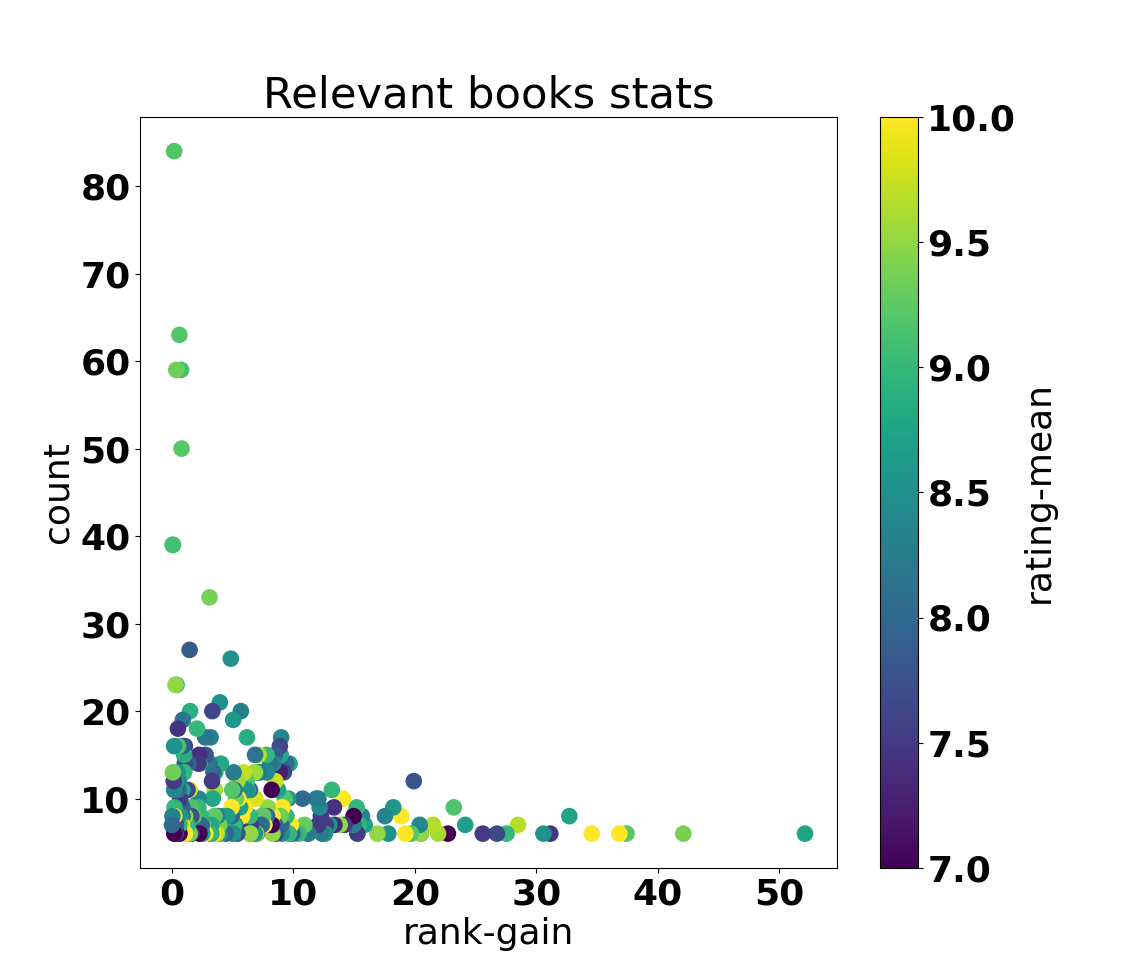
\includegraphics[width=0.6\textwidth]{../img/rank-scatter.png}
		\caption{Scatter plot of Tolkien co-rated book metrics}
	\end{figure}
	Note that we could select books for further analysis in different ways. Prefering those with highest rank gain, those with high count, or some sort of combined multi-objective (Pareto) selection.
\end{frame}

\section{Book groups}

\begin{frame}{Linking}
	Build a graph of links between books with positive ranking gain
	\begin{itemize}
		\item create set of most common Tolkien books $\{\tau_k\}$ and positive rank gain books $\{\rho_l\}$, $\{\mu_m\}=\{\tau_k\}\cup\{\rho_l\}$
		\item count pair-wise co-ocurrence in the same rating group $\gamma_i$ for each pair $(\mu_m,\mu_n)$
		\item get symmetric matrix of co-ocurrence, naming $\rho{-}\rho$ co-occurences $R$, $\tau{-}\tau$ co-occurences $T$, and $\rho{-}\tau$ co-occurences $Q$
	\end{itemize}
\end{frame}


\begin{frame}{Getting linked group}
	Estimate a group of books linked to LOTR books and to one another
	\begin{itemize}
		\item create a normalized vector of weights $\tau^{(1)}$ as relative LOTR books count
		\item compute a vector of non-LOTR books linked ($\rho{-}\tau$ co-ocurrence) to this vector, $\rho^{(1)}$
		\item redistribute weights $\rho^{(n-1)} \rightarrow \rho^{(n)}$  by links between the books while weight std grows, until vector converges
		\item select the top books from $\rho^{(n)}$
	\end{itemize}
	\\[1em]
	\begin{equation*}
		\begin{bmatrix}
			\rho^{(1)} \\
			0
		\end{bmatrix}
		=
		\begin{bmatrix}
			R & Q \\
			Q^T  & T
		\end{bmatrix}
		\begin{bmatrix}
			0  \\
			\tau^{(1)}
		\end{bmatrix}
	\end{equation*}	
	\\[1em]
	\begin{equation*}
		\begin{bmatrix}
			\rho^{(n)}
		\end{bmatrix}
		= R
		\begin{bmatrix}
			\rho^{(n-1)}
		\end{bmatrix}
	\end{equation*}
\end{frame}


\end{document}
